\section{Preliminaries: Model, Mechanism, and Assumptions}
\label{sec:preliminaries}

This section sets up the model of \textcite{srinivasan2025selfresolving} that our
experiments are built on. We keep the notation light and refer to the original paper
for full proofs.

\subsection{Setting}

The goal is to elicit and aggregate probabilistic predictions about a binary outcome
$Y \in \{0,1\}$ (categorical and discretised-continuous outcomes reduce to this case).
There are $M$ agents who arrive \emph{one at a time}. Agent $t$ has a private signal
$X^{(t)}$ drawn from a common prior $\mathbb{P}(Y, X^{(1)}, \dots, X^{(M)})$ and, on
arrival, also observes all previous reports $\mathbf{q}^{(1:t-1)}$. Conditioning on
$\hat X^{(t)} = \{X^{(t)}, \mathbf{q}^{(1:t-1)}\}$, the agent forms a posterior
$\bar{\mathbf p}^{(t)} = \mathbb{P}(Y \mid \hat X^{(t)})$ and reports some
$\mathbf{q}^{(t)} \in \Delta\Omega_Y$ to the mechanism. A truthful agent reports
$\mathbf{q}^{(t)} = \bar{\mathbf p}^{(t)}$; a strategic agent may report something else.

We write $y_1 = \mathbb{P}(Y=1)$ and $y_0 = 1-y_1$ for the prior, and use $t$ for the
agent under consideration and $r$ for its \emph{reference agent}.

\subsection{Scoring rules: from outcome to reference}

A proper scoring rule $S(i, \mathbf{q})$ rewards a probabilistic report
$\mathbf{q}$ against a realised outcome $i$, and is \emph{proper} when reporting one's
true belief maximises expected reward~\parencite{gneiting2007strictly}. The canonical
choice is the \emph{log scoring rule} $S(i, \mathbf{q}) = \log q_i$, which underlies
the cross-entropy rule used throughout the paper. The crucial move is to score a
report against another \emph{prediction} $\mathbf{r} \in \Delta\Omega_Y$ instead of an
outcome:
\begin{equation}
    S_{CE}(\mathbf{r}, \mathbf{q}) = -H(\mathbf{r}, \mathbf{q}) = \sum_i r_i \log q_i .
    \label{eq:ce}
\end{equation}
Because an agent does not know what the reference will report, it maximises its
\emph{expected} cross-entropy, which is maximised by reporting its expectation of the
reference's prediction, $\mathbb{E}[\mathbf{r}]$. The mechanism uses the sequential,
shared version of this rule --- the \emph{cross-entropy market scoring rule (CE-MSR)} ---
which pays an agent for how much it \emph{improves} the running forecast relative to
the reference:
\begin{equation}
    S_{CEM}(\mathbf{r}, \mathbf{q}^{(t)}, \mathbf{q}^{(t-1)})
    = -H(\mathbf{r}, \mathbf{q}^{(t)}) + H(\mathbf{r}, \mathbf{q}^{(t-1)})
    = \sum_i r_i \log\!\left(\frac{q^{(t)}_i}{q^{(t-1)}_i}\right).
    \label{eq:cemsr}
\end{equation}
Intuitively, \eqref{eq:cemsr} asks: \emph{how much closer to the reference is the new
report than the previous one?} Swapping the outcome $i$ in $\log q_i$ for a reference
$\mathbf{r}$ in \eqref{eq:ce} is precisely what lets the market resolve without an
outcome.

\subsection{The self-resolving mechanism}

The mechanism (Figure~\ref{fig:mechanism}) proceeds as follows:
\begin{enumerate}
    \item Agents $1, 2, \dots$ arrive in sequence; agent $t$ observes the history
    $\mathbf{q}^{(1:t-1)}$ and its signal $X^{(t)}$, and reports $\mathbf{q}^{(t)}$.
    \item After each report the market \emph{terminates with probability $\alpha$}.
    Let $T$ be the (random) terminal time. The terminal agent $T$ is the
    \textbf{reference agent} $r$: having seen the whole history, it is the
    best-informed participant.
    \item Agents $1, \dots, T-k$ are paid the CE-MSR \eqref{eq:cemsr} against the
    reference's report $\mathbf{q}^{(T)}$. The last $k$ agents (those too close to the
    reference) instead receive a flat fee $R$, so they cannot be paid to manipulate a
    reference that they themselves heavily influence.
\end{enumerate}
The single design parameter $k$ controls how far an agent must be from the reference
to be scored against it; larger $k$ means a better-informed reference relative to any
single scored agent, at the cost of paying more agents the flat fee.

\begin{figure}[H]
    \centering
    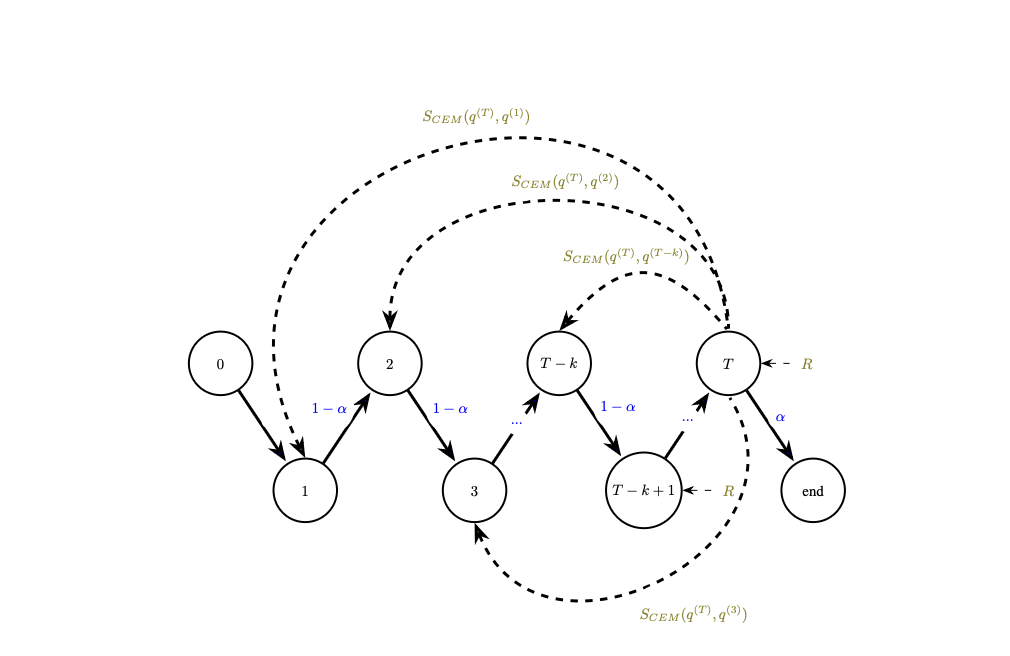
\includegraphics[width=0.9\linewidth]{Images/srpm_mechanism.png}
    \caption[The self-resolving prediction market mechanism]{The self-resolving
    prediction market. Each node is an agent reporting to the mechanism; the market
    terminates with probability $\alpha$ after each report. The first $T-k$ agents are
    paid the cross-entropy market scoring rule against the terminal reference agent
    $T$, while the last $k$ agents receive a flat fee $R$. Redrawn after
    \textcite{srinivasan2025selfresolving}, Figure~1.}
    \label{fig:mechanism}
\end{figure}

\subsection{Assumptions}
\label{subsec:assumptions}

The mechanism's guarantees rest on five assumptions about agents and signals. They
matter for us because our two studies are organised precisely around when they hold
and when they do not.
\begin{description}
    \item[\textbf{A1 (Rationality \& risk-neutrality).}] Agents are risk-neutral,
    fully rational Bayesians, and this is common knowledge.
    \item[\textbf{A2 (Common prior).}] Signals and outcome are drawn from a common
    prior that is common knowledge.
    \item[\textbf{A3 (Stochastic relevance / distinct signals).}] Each signal induces
    a \emph{unique} posterior over $Y$, so agents can invert one another's reports back
    into the underlying signal.
    \item[\textbf{A4 (Conditional independence).}] Signals are independent given $Y$ ---
    i.e.\ they are informational \emph{substitutes}~\parencite{chen2016informational}.
    This is the same class of information structures under which \emph{standard}
    prediction markets are incentive-compatible~\parencite{chen2010gaming}.
    \item[\textbf{A5 ($(\delta,\eta)$-informative signals).}] Two floors on signal
    informativeness: $\delta$ lower-bounds how much each signal separates $Y=0$ from
    $Y=1$ (via the Bhattacharyya coefficient, $BC \le 1-\delta$), and $\eta$
    lower-bounds every signal likelihood, $\min_{x,\omega}\mathbb{P}(X=x\mid Y=\omega)\ge\eta$,
    so no single report can be arbitrarily decisive.
\end{description}
Two derived quantities recur below. The \emph{Bhattacharyya coefficient}
$BC = \sum_i \sqrt{\mathbb{P}(X_i\mid Y{=}0)\,\mathbb{P}(X_i\mid Y{=}1)} = 1-\delta$
measures the overlap between the two conditional signal distributions ($\delta = 0$ is
a useless signal, larger $\delta$ a more separating one). The \emph{$\tau$-granularity}
is the smallest gap between the log-likelihood ratios of two distinct signals, which
controls how strictly an agent prefers truthful reporting.

\subsection{What the paper proves}
\label{subsec:guarantees}

Three results, all expressing the same idea --- \emph{a well-informed reference makes
honesty optimal} --- frame our experiments:
\begin{itemize}
    \item \textbf{Theorem 1 (bounded influence).} If the reference observes $k$
    informational substitutes that agent $t$ does not, then $t$'s influence on the
    reference's posterior --- the adjustment term $\Delta$ --- shrinks geometrically,
    $|\Delta| \le \tfrac14\!\left(\tfrac{1-\eta}{\eta}-\tfrac{\eta}{1-\eta}\right)(1-\delta)^k$.
    Enough substitutes $\Rightarrow$ the reference is effectively ground truth.
    \item \textbf{Theorem 2 (strict truthfulness).} Paid by CE-MSR against a truthful
    reference, agent $t$ \emph{strictly} maximises expected payoff by reporting
    truthfully once the reference has at least an explicit threshold number of signals
    (in $\delta, \eta, \tau$ and the prior).
    \item \textbf{Theorem 3 (vanishing gain from deviation).} The gain from \emph{any}
    deviation is bounded by a function $\hat D_\eta(\Delta, \mathbf{y})$ of the
    adjustment $\Delta$; since $\Delta \to 0$ as $k$ grows (Theorem~1), this bound
    $\to 0$ --- and, crucially, without needing to know $\tau$.
\end{itemize}
Theorem~1 motivates the analytic minimum-substitutes quantity $k_{\min}$ that we
reproduce in Section~\ref{sec:methods}, and Theorem~3 is exactly the prediction our
simulation tests: the profit-maximising deviation should collapse onto truthful
reporting as $k$ grows.

\subsection{Problem statement and research questions}

The original paper stops at these guarantees. Our problem is to give them empirical
content and to probe their boundaries, through two questions:
\begin{description}
    \item[\textbf{RQ1 (incentives, simulation).}] In a world where A1--A4 hold by
    construction, when does a freely deviating agent actually find truthful reporting
    to be a best response, and how does this depend on how informed the reference is
    (the one assumption, A5, that we vary)?
    \item[\textbf{RQ2 (robustness, empirical).}] On real resolved markets --- where
    essentially none of A1--A5 hold --- how closely do self-resolving payouts track the
    standard verifiable (outcome-based) payouts they are designed to replace?
\end{description}
